% Options for packages loaded elsewhere
\PassOptionsToPackage{unicode}{hyperref}
\PassOptionsToPackage{hyphens}{url}
\PassOptionsToPackage{dvipsnames,svgnames,x11names}{xcolor}
%
\documentclass[
]{agujournal2019}

\usepackage{amsmath,amssymb}
\usepackage{iftex}
\ifPDFTeX
  \usepackage[T1]{fontenc}
  \usepackage[utf8]{inputenc}
  \usepackage{textcomp} % provide euro and other symbols
\else % if luatex or xetex
  \usepackage{unicode-math}
  \defaultfontfeatures{Scale=MatchLowercase}
  \defaultfontfeatures[\rmfamily]{Ligatures=TeX,Scale=1}
\fi
\usepackage{lmodern}
\ifPDFTeX\else  
    % xetex/luatex font selection
\fi
% Use upquote if available, for straight quotes in verbatim environments
\IfFileExists{upquote.sty}{\usepackage{upquote}}{}
\IfFileExists{microtype.sty}{% use microtype if available
  \usepackage[]{microtype}
  \UseMicrotypeSet[protrusion]{basicmath} % disable protrusion for tt fonts
}{}
\makeatletter
\@ifundefined{KOMAClassName}{% if non-KOMA class
  \IfFileExists{parskip.sty}{%
    \usepackage{parskip}
  }{% else
    \setlength{\parindent}{0pt}
    \setlength{\parskip}{6pt plus 2pt minus 1pt}}
}{% if KOMA class
  \KOMAoptions{parskip=half}}
\makeatother
\usepackage{xcolor}
\setlength{\emergencystretch}{3em} % prevent overfull lines
\setcounter{secnumdepth}{5}
% Make \paragraph and \subparagraph free-standing
\ifx\paragraph\undefined\else
  \let\oldparagraph\paragraph
  \renewcommand{\paragraph}[1]{\oldparagraph{#1}\mbox{}}
\fi
\ifx\subparagraph\undefined\else
  \let\oldsubparagraph\subparagraph
  \renewcommand{\subparagraph}[1]{\oldsubparagraph{#1}\mbox{}}
\fi

\usepackage{color}
\usepackage{fancyvrb}
\newcommand{\VerbBar}{|}
\newcommand{\VERB}{\Verb[commandchars=\\\{\}]}
\DefineVerbatimEnvironment{Highlighting}{Verbatim}{commandchars=\\\{\}}
% Add ',fontsize=\small' for more characters per line
\usepackage{framed}
\definecolor{shadecolor}{RGB}{241,243,245}
\newenvironment{Shaded}{\begin{snugshade}}{\end{snugshade}}
\newcommand{\AlertTok}[1]{\textcolor[rgb]{0.68,0.00,0.00}{#1}}
\newcommand{\AnnotationTok}[1]{\textcolor[rgb]{0.37,0.37,0.37}{#1}}
\newcommand{\AttributeTok}[1]{\textcolor[rgb]{0.40,0.45,0.13}{#1}}
\newcommand{\BaseNTok}[1]{\textcolor[rgb]{0.68,0.00,0.00}{#1}}
\newcommand{\BuiltInTok}[1]{\textcolor[rgb]{0.00,0.23,0.31}{#1}}
\newcommand{\CharTok}[1]{\textcolor[rgb]{0.13,0.47,0.30}{#1}}
\newcommand{\CommentTok}[1]{\textcolor[rgb]{0.37,0.37,0.37}{#1}}
\newcommand{\CommentVarTok}[1]{\textcolor[rgb]{0.37,0.37,0.37}{\textit{#1}}}
\newcommand{\ConstantTok}[1]{\textcolor[rgb]{0.56,0.35,0.01}{#1}}
\newcommand{\ControlFlowTok}[1]{\textcolor[rgb]{0.00,0.23,0.31}{#1}}
\newcommand{\DataTypeTok}[1]{\textcolor[rgb]{0.68,0.00,0.00}{#1}}
\newcommand{\DecValTok}[1]{\textcolor[rgb]{0.68,0.00,0.00}{#1}}
\newcommand{\DocumentationTok}[1]{\textcolor[rgb]{0.37,0.37,0.37}{\textit{#1}}}
\newcommand{\ErrorTok}[1]{\textcolor[rgb]{0.68,0.00,0.00}{#1}}
\newcommand{\ExtensionTok}[1]{\textcolor[rgb]{0.00,0.23,0.31}{#1}}
\newcommand{\FloatTok}[1]{\textcolor[rgb]{0.68,0.00,0.00}{#1}}
\newcommand{\FunctionTok}[1]{\textcolor[rgb]{0.28,0.35,0.67}{#1}}
\newcommand{\ImportTok}[1]{\textcolor[rgb]{0.00,0.46,0.62}{#1}}
\newcommand{\InformationTok}[1]{\textcolor[rgb]{0.37,0.37,0.37}{#1}}
\newcommand{\KeywordTok}[1]{\textcolor[rgb]{0.00,0.23,0.31}{#1}}
\newcommand{\NormalTok}[1]{\textcolor[rgb]{0.00,0.23,0.31}{#1}}
\newcommand{\OperatorTok}[1]{\textcolor[rgb]{0.37,0.37,0.37}{#1}}
\newcommand{\OtherTok}[1]{\textcolor[rgb]{0.00,0.23,0.31}{#1}}
\newcommand{\PreprocessorTok}[1]{\textcolor[rgb]{0.68,0.00,0.00}{#1}}
\newcommand{\RegionMarkerTok}[1]{\textcolor[rgb]{0.00,0.23,0.31}{#1}}
\newcommand{\SpecialCharTok}[1]{\textcolor[rgb]{0.37,0.37,0.37}{#1}}
\newcommand{\SpecialStringTok}[1]{\textcolor[rgb]{0.13,0.47,0.30}{#1}}
\newcommand{\StringTok}[1]{\textcolor[rgb]{0.13,0.47,0.30}{#1}}
\newcommand{\VariableTok}[1]{\textcolor[rgb]{0.07,0.07,0.07}{#1}}
\newcommand{\VerbatimStringTok}[1]{\textcolor[rgb]{0.13,0.47,0.30}{#1}}
\newcommand{\WarningTok}[1]{\textcolor[rgb]{0.37,0.37,0.37}{\textit{#1}}}

\providecommand{\tightlist}{%
  \setlength{\itemsep}{0pt}\setlength{\parskip}{0pt}}\usepackage{longtable,booktabs,array}
\usepackage{calc} % for calculating minipage widths
% Correct order of tables after \paragraph or \subparagraph
\usepackage{etoolbox}
\makeatletter
\patchcmd\longtable{\par}{\if@noskipsec\mbox{}\fi\par}{}{}
\makeatother
% Allow footnotes in longtable head/foot
\IfFileExists{footnotehyper.sty}{\usepackage{footnotehyper}}{\usepackage{footnote}}
\makesavenoteenv{longtable}
\usepackage{graphicx}
\makeatletter
\def\maxwidth{\ifdim\Gin@nat@width>\linewidth\linewidth\else\Gin@nat@width\fi}
\def\maxheight{\ifdim\Gin@nat@height>\textheight\textheight\else\Gin@nat@height\fi}
\makeatother
% Scale images if necessary, so that they will not overflow the page
% margins by default, and it is still possible to overwrite the defaults
% using explicit options in \includegraphics[width, height, ...]{}
\setkeys{Gin}{width=\maxwidth,height=\maxheight,keepaspectratio}
% Set default figure placement to htbp
\makeatletter
\def\fps@figure{htbp}
\makeatother
% definitions for citeproc citations
\NewDocumentCommand\citeproctext{}{}
\NewDocumentCommand\citeproc{mm}{%
  \begingroup\def\citeproctext{#2}\cite{#1}\endgroup}
\makeatletter
 % allow citations to break across lines
 \let\@cite@ofmt\@firstofone
 % avoid brackets around text for \cite:
 \def\@biblabel#1{}
 \def\@cite#1#2{{#1\if@tempswa , #2\fi}}
\makeatother
\newlength{\cslhangindent}
\setlength{\cslhangindent}{1.5em}
\newlength{\csllabelwidth}
\setlength{\csllabelwidth}{3em}
\newenvironment{CSLReferences}[2] % #1 hanging-indent, #2 entry-spacing
 {\begin{list}{}{%
  \setlength{\itemindent}{0pt}
  \setlength{\leftmargin}{0pt}
  \setlength{\parsep}{0pt}
  % turn on hanging indent if param 1 is 1
  \ifodd #1
   \setlength{\leftmargin}{\cslhangindent}
   \setlength{\itemindent}{-1\cslhangindent}
  \fi
  % set entry spacing
  \setlength{\itemsep}{#2\baselineskip}}}
 {\end{list}}
\usepackage{calc}
\newcommand{\CSLBlock}[1]{\hfill\break\parbox[t]{\linewidth}{\strut\ignorespaces#1\strut}}
\newcommand{\CSLLeftMargin}[1]{\parbox[t]{\csllabelwidth}{\strut#1\strut}}
\newcommand{\CSLRightInline}[1]{\parbox[t]{\linewidth - \csllabelwidth}{\strut#1\strut}}
\newcommand{\CSLIndent}[1]{\hspace{\cslhangindent}#1}

\usepackage{url} %this package should fix any errors with URLs in refs.
\usepackage{lineno}
\usepackage[inline]{trackchanges} %for better track changes. finalnew option will compile document with changes incorporated.
\usepackage{soul}
\linenumbers
\makeatletter
\@ifpackageloaded{caption}{}{\usepackage{caption}}
\AtBeginDocument{%
\ifdefined\contentsname
  \renewcommand*\contentsname{Table of contents}
\else
  \newcommand\contentsname{Table of contents}
\fi
\ifdefined\listfigurename
  \renewcommand*\listfigurename{List of Figures}
\else
  \newcommand\listfigurename{List of Figures}
\fi
\ifdefined\listtablename
  \renewcommand*\listtablename{List of Tables}
\else
  \newcommand\listtablename{List of Tables}
\fi
\ifdefined\figurename
  \renewcommand*\figurename{Figure}
\else
  \newcommand\figurename{Figure}
\fi
\ifdefined\tablename
  \renewcommand*\tablename{Table}
\else
  \newcommand\tablename{Table}
\fi
}
\@ifpackageloaded{float}{}{\usepackage{float}}
\floatstyle{ruled}
\@ifundefined{c@chapter}{\newfloat{codelisting}{h}{lop}}{\newfloat{codelisting}{h}{lop}[chapter]}
\floatname{codelisting}{Listing}
\newcommand*\listoflistings{\listof{codelisting}{List of Listings}}
\makeatother
\makeatletter
\makeatother
\makeatletter
\@ifpackageloaded{caption}{}{\usepackage{caption}}
\@ifpackageloaded{subcaption}{}{\usepackage{subcaption}}
\makeatother
\ifLuaTeX
  \usepackage{selnolig}  % disable illegal ligatures
\fi
\usepackage{bookmark}

\IfFileExists{xurl.sty}{\usepackage{xurl}}{} % add URL line breaks if available
\urlstyle{same} % disable monospaced font for URLs
\hypersetup{
  pdftitle={How Does Customer Feedback Vary Across Leading Airline Review Platforms?},
  pdfauthor={Adeim Suvanbekova; Christian González-Martel; Teresa Aguiar-Quintana},
  pdfkeywords={Bayesian Hierarchical Model, Online Consumer Reviews
(OCRs), Airline Service Quality},
  colorlinks=true,
  linkcolor={blue},
  filecolor={Maroon},
  citecolor={Blue},
  urlcolor={Blue},
  pdfcreator={LaTeX via pandoc}}

\journalname{Hospitality}

\draftfalse

\begin{document}
\title{How Does Customer Feedback Vary Across Leading Airline Review
Platforms?}

\authors{Adeim Suvanbekova\affil{1,2}, Christian
González-Martel\affil{3}, Teresa Aguiar-Quintana\affil{4,2}}
\affiliation{1}{Universidad de Las Palmas de Gran
Canaria, }\affiliation{2}{TIDES Institute, }\affiliation{3}{Department
of Quantitative Methods in Economics, Universidad de Las Palmas de Gran
Canaria, }\affiliation{4}{Department of Economics and Business
Management, Universidad de Las Palmas de Gran Canaria, }
\correspondingauthor{Teresa Aguiar-Quintana}{}


\begin{abstract}
This study investigates score heterogeneity in online consumer reviews
(OCRs) for airlines across TripAdvisor and Skytrax. The research
addresses the variability in review scores, focusing on two airlines:
Ryanair and Lufthansa. Previous studies have largely ignored
cross-platform score variability, and this study fills that gap by
applying a Bayesian hierarchical model. This model is suitable for its
ability to incorporate prior knowledge and handle complex data
structures. The dataset spans from January 1, 2023, to December 31,
2023. Results indicate no significant differences in review scores
between platforms or airlines, suggesting consistent customer
satisfaction. However, a significant interaction effect between
TripAdvisor and Ryanair indicates lower scores for this combination.
These findings highlight the importance of platform-airline interactions
in customer feedback analysis. The study's implications underscore the
need for tailored strategies in managing OCRs and validate the use of
Bayesian methodologies in hospitality research. Future research should
expand the dataset for broader validation.
\end{abstract}

\section*{Plain Language Summary}
This study looks at how customer reviews for airlines differ between
TripAdvisor and Skytrax. We analyzed reviews for Ryanair and Lufthansa
using a special statistical method to see if there are big differences
in ratings. We found that, on average, ratings are similar across both
platforms and airlines. However, Ryanair reviews on TripAdvisor tend to
be lower. These findings can help airlines understand and improve their
online reputation.



\section{Introduction}\label{introduction}

As technology continues to advance industries globally and
digitalization transforms operations, the hospitality sector has
undergone significant changes. This evolution , driven by Web 2.0
technologies, has given rise to online review platforms featuring
user-generated content (UGC), providing valuable insights for
prospective customers and fundamentally reshaping customer engagement
with businesses. Thus, online consumer reviews (OCRs) have begun to
significantly influence consumer decision-making processes (Mendes-Filho
et al., 2018), shaping brand image (Lam et al., 2020) , and enhancing
electronic Word-of-Mouth (eWOM) (Muda \& Hamzah, 2021; Nusairat et al.,
2021). Furthermore, within the academic field, scholars are increasingly
recognizing the advantages of applying UGC due to its accessibility and
capacity for in-depth analysis. Consequently, there has been a notable
growth in scholarly research incorporating UGC.

Given the unique characteristics of airline services, both in-flight and
on-ground, effective customer communication and feedback are indicators
of the operational efficiency and overall customer experience. Existing
literature on airline services heavily relies on surveys as the primary
data source to explore perceptions of service quality and customer
satisfaction. The recent increasing integration of online reviews into
scholarly research is attributed to accessibility, diverse perspectives,
and rich data content, thereby overcoming the sampling limitations
associated with traditional surveys. The incorporation of UGC within the
airline industry has been widely utilized for various research aims,
such as assessing passengers' emotions following flight delays (Song et
al., 2020), investigating the impact of airline alliance strategy on
service quality (Migdadi, 2022), and predicting airline recommendations.
(Jain et al., 2022; Siering et al., 2018). However, despite the growing
literature utilizing custom-shared experiences, there remains a gap in
understanding the variability in online customer ratings within the
airline industry. To address this gap, this study proposes a Bayesian
approach for measuring and managing score heterogeneity across major
online review platforms.

\textbf{(Methodogy/Need to check)} Recently, (Martel--Escobar et al.,
2023) noted a lack of research on the application of Bayesian techniques
in publications within the tourism and hospitality sectors, particularly
in studies focused on eWOM. While Bayesian approaches have found
extensive adoption across various fields such as finance, healthcare,
and marketing over the past decades, their application in hospitality
research remains limited. Despite numerous advantages, including the
incorporation of prior data, flexibility, and the ability to handle
small sample sizes, the integration of Bayesian methods in hospitality
studies remains constrained. According to Bianchi \& Heo (2021) Bayesian
statistics provide a more nuanced analysis compared to classical
methods, which is particularly beneficial for the hospitality sector.
Through the analysis of data obtained from primary OCR platforms for
airlines, namely TripAdvisor and Skytrax, the study presents a novel
Bayesian approach to understanding score heterogeneity among the
principal review portals for airlines.

The airline industry has experienced notable transformations following
the introduction of Low-Cost Carriers (LCCs), which have impacted
passengers' perceptions and shaped distinct expectations according to
airline's business model. The evaluation of services provided by LCCs
differ compared to Full-Service Carriers (FSCs) due to disparities in
airfare pricing and customer anticipations. This distinction is
underscored by the customer satisfaction coefficient, revealing the
heightened importance of different attributes (Byun \& Lee, 2016). Thus,
to conduct a comprehensive analysis, both LCCs and FSCs will be
examined.

Given research presents the methodology and findings of Bayesian
analysis, based on data collected from leading online review platforms
for both LCCs and FSCs. Through in-depth approach, the study not only
contributes to the existing literature on UGC and airline service
quality but also brings attention to rating heterogeneity, offering a
comprehensive understanding of score variations. These insights are
valuable for theoretical scholars utilizing UGC for their analysis, as
the majority of studies tend to concentrate on a single UGC platform,
while also holding practical implications for stakeholders seeking to
enhance service quality, foster eWOM, and manage brand image effectively
within the highly competitive industry.

\section{Literature Review}\label{sec-lit-review}

\subsection{The importance of online consumer reviews in
tourism.}\label{the-importance-of-online-consumer-reviews-in-tourism.}

Online reviews have captured considerable attention of both academia and
industry due to their significant impact on consumer behavior and
purchasing decisions. Thus, UGC has become increasingly essential in the
tourism sector, particularly considering the intangible nature of
hospitality and the growing reliance on reviews for travel planning.
Notably, such content is considered more credible than official sites
and tourist destination pages (Bilos et al., 2022), influences
travelers' behavior more than marketing-generated-content (Tsiakali,
2018), and positively influences tourists' intentions to book a hotel
and visit a destination (Ukpabi \& Karjaluoto, 2018). Research by Cox et
al. (2009) in the accommodation sector reveals that the majority of
consumers prioritize the views of other travelers over the hotel's
self-description available online. Furthermore, UGC has more credibility
and trustworthiness compared to professionally generated content, and
this trustworthiness remains consistent regardless of whether
participants encounter positive or negative information (Cheong \&
Morrison, 2008).

According to Muritala et al. (2020), the research on online reviews and
electronic eWOM in tourism and hospitality is reaching a mature stage,
characterized by a rapidly growing volume of studies built on a solid
base of seminal research and the application of the latest analytical
techniques, including artificial neural networks and deep learning.
Academics have extensively studied UGC in relation to travel planning
behaviour (Bilos et al., 2022; Cox et al., 2009; Mendes-Filho et al.,
2018; Tsiakali, 2018), corporate reputation management (Baka, 2016;
Nicoli \& Papadopoulou, 2017), motivations for content contribution
(Bronner \& Hoog, 2011; Daugherty et al., 2008; Kaur \& Singh, 2021; Yoo
\& Gretzel, 2009), credibility perception (Cheong \& Morrison, 2008;
Filieri et al., 2021; Lo \& Yao, 2019), helpfulness determinants
(Filieri et al., 2021; Hu \& Yang, 2020; Huang et al., 2015; Kwon et
al., 2021; Lo \& Yao, 2019), predicting recommendations (Jain et al.,
2022; Siering et al., 2018), and service recovery (Etemad-Sajadi \&
Bohrer, 2019; Xu et al., 2019).

The increasing adoption of OCRs in scholarly research is attributed to
numerous advantages. Firstly, it provides direct access to extensive
datasets with organically generated and diverse data. In certain
instances, OCRs enable researchers to gather socio-demographic details
of content contributors, supporting cross-cultural studies and analyses
of age or gender disparities (Dike et al., 2024; Punel et al., 2019;
Stamolampros et al., 2019; Sudhakar \& Gunasekar, 2020). \textbf{(DO I
NEED TO PUT ARTICLES?)}. Additionally, given the unique nature of
airline services, reviews often contain valuable information on cabin
class, airline type, and routes for evaluating moderating effect and
comparative analysis, along with additional ratings on certain service
attributes for extended examination (Lucini et al., 2020; Sezgen et al.,
2019; Tahanisaz \& shokuhyar, 2020). Furthermore, reviews allow
researchers to track changes in customer perceptions, preferences, and
behaviors in response to significant external factors such as the
COVID-19 pandemic (Hassan \& Salem, 2022; Nilashi et al., 2022; Sulu et
al., 2022) and economic crises. However, study by W. Lu \& Stepchenkova
(2015) underscores that the anonymity of UGC creators, sample
representativeness and the generalizability of results poses challenges
to research validity, thereby questioning the reliability of findings.

Acknowledging the importance of online reviews, scholars have begun
investigating their credibility and willingness to use. Research
conducted by Lo \& Yao (2019) revealed higher perceived credibility
scores among reviews that are negative , written by experts and with a
consistent rating. Consumers seek the opinions of others to minimize
risks and gather prepurchase information, making these opinions more
valuable than advertising. According to Bilos et al. (2022) respondents
rely on UGC more than their friends' recommendations and promotional
content. For analyzing the intention to use online consumer reviews,
scholars rely on the Technology Acceptance Model (TAM) (Davis, 1989) as
a predominant framework in hospitality literature, which identifies
perceived usefulness and ease of use as key factors. In addition,
Changchit et al. (2020) identified perceived credibility and importance
of online reviews, along with computer self-efficacy, as additional
factors influencing users' intentions. According to Mendes-Filho et al.
(2018), there is a heightened intention to use UGC in travel planning if
the content provides perceived empowerment and usefulness. The study by
Assaker (2020) found that gender and age significantly moderate
travellers' intention to use UGC, with perceived usefulness being more
influential for male travellers and perceived ease of use being more
impactful for female and older travellers.

Online travel review authors are primarily motivated by a desire to help
service providers, concern for other consumers, and the need for
enjoyment and positive self-enhancement (Yoo \& Gretzel, 2009). Kaur \&
Singh (2021) analysing motivations behind review submission, defined
altruism, reciprocity, egocentric behavior, knowledge self-efficacy, and
collectivism as a key antecedents. Identifying profile of vacationers
contributing to review sites, Bronner \& Hoog (2011) reveal them to
typically be under 55 years, from high and lower-middle-income groups,
and often couples with or without children. The authors highlighted the
importance of distinguishing between self-directed and other-directed
motivations, which influence the type of review site and the manner of
expression. Self-directed motivations favor marketer-generated sites,
commenting on fewer aspects, predominantly negative reviews, and
contributing to less accessible platforms. Vacationers with
other-directed motivations prefer consumer-generated sites, engaging in
broader commenting, posting mainly positive reviews, using both text and
ratings, and contributing to sites accessible to other vacationers.
According to Wilson et al. (2012), national attitudes and motivations
significantly influence the type of UGC posted. In their study, authors
found that British and Swiss users tend to share photos and videos on
social media to relive vacation experiences, while Spanish users prefer
using text and comments to make recommendations to other travelers.

With the widespread availability of online reviews and the consequent
information overload, scholars have begun to study reviews in relation
to their perceived helpfulness. However, despite extensive research into
the determinants of review helpfulness within tourism and hospitality,
findings remain mixed. A recent study by Hu \& Yang (2020) identified
review length as the most influential factor, followed by reviewer
expertise and age, while the impact of review valence and readability
was found to be insignificant. Conversely, Filieri et al. (2018)
contended that long reviews are not necessarily perceived as helpful.
Instead, consumers favor fact-based, objective, and logically structured
reviews especially in the context of high involvement purchase
decisions. According to Kwok \& Xie (2016), the helpfulness of online
hotel reviews is negatively affected by review length and rating,
whereas positively impacted by manager response and reviewer experience.
Huang et al. (2015) determined the relationship between word count and
helpfulness remained significant for reviews containing 144 words or
fewer. However, once the word count exceeded, the relationship loose
statistical significance. Analysing extremely negative ratings, Filieri
et al. (2019), found that these ratings are often considered helpful and
diagnostic, as they provide valuable insights to justify the extreme
evaluation, thereby significantly contributing to consumer
decision-making.

\subsection{The research on OCR applied to airlines
industry}\label{the-research-on-ocr-applied-to-airlines-industry}

Despite the growing adoption of reviews in scholarly research, studies
specifically addressing online reviews related to airlines remain
limited. Analyzing service quality within tourism and hospitality
industry using UGC, W. Lu \& Stepchenkova (2015) discovered that the
majority of studies focused on the lodging setting, with relatively
fewer investigations conducted in the airline, online travel agent, and
restaurant settings. Similarly, an analysis of online customer
evaluations in tourism and hospitality by Schuckert et al. (2015)
revealed that over half of the reviewed articles concentrated on hotels.
Existing research of airline service through online customer-shared
experiences are primarily focused on perceptions of service quality
(Brochado et al., 2023; Korfiatis et al., 2019; Rasool \& Pathania,
2021), customer satisfaction (Ban \& Kim, 2019; Chatterjee et al., 2023;
Dike et al., 2024; Lucini et al., 2020), and behavioural intentions
(Siering et al., 2018; Wang et al., 2023).

Consumer feedback platforms have undergone a significant expansion,
gaining increasing popularity with the advent of Web 2.0. Online reviews
assessing airline services within the scholarly literature primarily
rely on data sourced from Skytrax and TripAdvisor platforms, with some
studies also incorporating UGC sourced from social media, particularly
Twitter. (DO I NEED TO ADD TWITTER ARTICLES). A study by L. Lu et al.
(2023) underscores the importance of incorporating content from multiple
review channels to gain a more accurate understanding of service
quality, recognizing the potential disparities across platforms. The
study on US airlines revealed that Skytrax reviewers prioritize boarding
and baggage experiences, whereas Twitter users emphasize customer
service interactions. Bilos et al. (2022) providing a comparative
analysis with Airbnb, found that TripAdvisor reviews are perceived as
more valuable for making purchasing decisions. Through conducting a
comparative analysis between results sourced from Twitter and the
Department of Transportation's official service quality report for US
airlines, (Tian et al., 2020) \textbf{SEARCH REFERENCE} established the
reliability of service quality metrics derived from social media.

Cross-cultural investigations in the field have uncovered differences in
the evaluation of provided services, influenced by the cultural
backgrounds of reviewers. Punel et al. (2019) revealed the influence of
passengers' country of residence to travel experience, perception, and
the evaluation of airline services. Notably, North American passengers
prioritize cost over in-flight services and complain more about their
national airlines, while East and Southeast Asian passengers are
satisfied with Asian airlines and value in-flight services. Middle
Easterners are critical of non-local airlines, while Oceania travelers
expect high service standards and South Americans have lower
expectations for in-flight amenities with an emphasis on price.
According to Dike and Davis (2023) \textbf{SEARCH REFERENCE} passengers
from individualistic cultural backgrounds tend to perceive service
quality as lower compared to customers from collectivist cultural
backgrounds. Stamolampros et al. (2019) found that airline passengers'
satisfaction with service quality varies depending on their cultural
values, impacting both overall satisfaction and specific aspects such as
staff interactions, food quality, seat comfort, and cleanliness.
Additionally, the study discovered that cultural characteristics
significantly shape both numerical ratings and textual content in
reviews.

The existing literature examining the airline industry underscores
distinct disparities between Low-Cost Carriers (LCCs) and Full-Service
Carriers (FSCs), emphasizing the significant impact of airline category
on passenger expectations and perceptions of service quality.
Consequently, each type of carrier should strategically prioritize
specific features to enhance overall service delivery. According to Lim
\& Lee (2020), FSCs should focus on enhancing tangible features, while
LCCs should concentrate on reliability. Furthermore, variations in
recommendation drivers exist across different airline business models.
(Siering et al., 2018) revealed that LCCs should focus on improving
augmented service aspects like amenities to enhance recommendations,
while FSNCs should prioritize core service aspects such as in-flight
amenities and customer service quality.

\subsubsection{OCR studies based on data collected in
Tripadvisor.}\label{ocr-studies-based-on-data-collected-in-tripadvisor.}

Tripadvisor, the world's largest travel guidance platform, features over
1 billion reviews and is accessible in 43 markets and 22 languages
(Tripadvisor, 2024) \textbf{SEARCH REFERENCE}. In addition to its
general community guidelines, the platform has established specific
posting guidelines for reviews, which are displayed on an organization's
listing page and are associated with a bubble rating ranging from 1 to
5. Beyond overall ratings, contributors evaluate additional service
attributes, including legroom, seat comfort, in-flight entertainment,
onboard experience, customer service, value for money, cleanliness,
check-in and boarding processes, as well as food and beverage quality.

The platform has been extensively utilized as a data source by various
investigators worldwide, contributing to diverse research findings. In
particular, online reviews serve as an efficient tool for examining
customer satisfaction. Sudhakar \& Gunasekar (2020) analyzed Indian
airlines using TripAdvisor feedbacks to reveal varying factors
influencing satisfaction across nationalities and airline types, with
Indian passengers prioritizing value for money and foreign passengers
prioritizing service attributes. Sezgen et al. (2019) examined 45
international airlines to define the key drivers of passenger
satisfaction and dissatisfaction across full-service and low-cost
carriers, as well as economy and premium cabins. Despite variations in
satisfaction drivers, fundamental factors such as friendly staff, value,
and service quality remain universally important. In the US airline
market, Park et al. (2020) underscores the need for sustainable
strategies beyond price competition, highlighting the asymmetric impact
of service quality attributes on customer satisfaction and their
critical importance in airline operations. According to Korfiatis et al.
(2019), integrating unstructured data from online reviews into service
quality assessment enhances understanding and predictability of customer
satisfaction. Examining Tripadvisor reviews, the study revealed temporal
variations in dimensions, thereby emphasizing the importance of
monitoring and adapting to changing customer preferences over time.

Additionally, Tripadvisor reviews have been used to identify key themes
by Brochado et al. (2019) and Sulu et al. (2022) during the pandemic.
The study by Brochado et al. (2019) was aimed to identify the main
themes in traveler reviews and their relationship with value-for-money
ratings by examining airlines affiliated with the largest alliances,
SkyTeam and Star Alliance, across France, the United States, Indonesia,
Canada, Taiwan, and Germany. Whereas, Sulu's (2022) research focused on
online airline reviews during the COVID-19 outbreak, aiming to define
principal themes and identify disparities among passengers of various
nationalities. The analysis revealed that European passengers exhibited
the most polarized opinions, ranging from highly critical to highly
satisfied, while American and Australian passengers predominantly
expressed positive reviews.

\subsubsection{OCR studies based on data collected in
Skytrax.}\label{ocr-studies-based-on-data-collected-in-skytrax.}

Skytrax is the international air transport rating organisation with Air
Travel review forum (www.airlinequality.com) that has become a leading
review site for airline, airport and associated air travel traveller
reviews \textbf{SEARCH REFERENCE} (Skytrax, 2024). Reviews submitted to
the platform undergo a multi-stage checking process to ensure compliance
with the Editorial Policy and requires reviewers to submit feedback that
follows a structured evaluation framework. The platform enables
passengers to share detailed opinions on their experiences across four
categories: airline, seat, airport, and lounge. Passengers can rate
airlines on a scale from 1 to 10 and provide textual comment, along with
additional details such as country of residence, date of flight, route,
cabin class, aircraft type, type of travel, and likelihood of
recommending the airline. Moreover, contributors assess supplementary
service attributes including value for money, ground service, seat
comfort, cabin staff service, food \& beverages, in-flight
entertainment, and cabin Wi-Fi \& connectivity.

Various scholars have used Skytrax reviews to define key factors
influencing customer experience and satisfaction within the airline
sector. Ban \& Kim (2019) identified six key clusters, including seat
comfort, staff service, entertainment, ground service, value for money,
and airline brand, with all factors except entertainment significantly
impacting customer satisfaction and recommendation. Shadiyar et
al.~(2020) \textbf{SEARCH REFERENCE} explored the utilization of big
data analytics and online customer reviews to enhance customer
satisfaction in airlines, identifying factors such as seat comfort,
staff behavior, food and beverage quality, ground service, and
particularly value for money as main. The study by Lucini et al. (2020)
was aimed to measure customer satisfaction by analyzing Skytrax reviews
to provide airlines with guidelines to improve competitiveness. The
study revealed that the type of cabin significantly impacts customer
satisfaction dimensions, prioritizing customer service for first-class
passengers, comfort for premium economy passengers, and efficient
baggage handling and minimal waiting times for economy class travellers,
whereas the type of passenger had minimal impact on satisfaction
dimensions. Dike et al. (2024) analyzed Skytrax feedbacks to explore how
customer culture, travel purpose, and seat type shape customer
expectations and satisfaction. The study highlighted that customer
service quality, delays, and baggage handling significantly impact
perceived service performance, with empathy and reliability having the
strongest influence on perceived satisfaction, while cultural
backgrounds affect levels of customer satisfaction. Chatterjee et al.
(2023) conducted a ten-year analysis of Skytrax reviews, identifying
core attributes such as value for money, seating comfort, and cabin
staff behaviour as more strongly related to customer satisfaction and
recommendation than augmented aspects like food and beverages and
in-flight entertainment. Authors found that core service attributes such
as responsiveness and reliability are crucial in shaping customer
satisfaction, whereas tangibles and empathy significantly influence
customers' likelihood of recommending an airline.

Also, Skytrax forum have been extensively used to analyze service
quality perceptions worldwide. Brochado's (2023) analysis of four
leading Chinese airlines highlighted value for money as consistently the
most influential service attribute, with varying responses from
different traveler types to service attributes. Kwon et al. (2021) used
the platform to understand customer needs and preferences in the Asian
airline market. Lim \& Lee (2020) used Skytrax feedbacks to compare
service quality perceptions between full-service carriers and low-cost
carriers , finding tangibles as the most significant dimension for FSCs
and reliability for LCCs. In terms of varied expectations of service
quality, Punel et al. (2019) revealed that different regions exhibit
distinct priorities and expectations concerning in-flight services and
overall satisfaction. Passengers in first or business class prioritize
seat comfort, food, and beverages, as well as in-flight entertainment.
In contrast, passengers in economy class place a higher emphasis on
value for money.

\textbf{The rest of this paper is organised as follows}

\section{Data \& Methods}\label{sec-data-methods}

\subsection{Bayesian Approach}\label{bayesian-approach}

This study adopts a Bayesian approach to analyze the score heterogeneity
of online consumer reviews (OCRs) across major airline review platforms,
specifically TripAdvisor and Skytrax.

Bayesian methods have been increasingly recognized in various fields for
their robustness in handling complex data structures and integrating
prior knowledge. The researcher starts with an initial belief about a
parameter (\(\theta\)) and its associated probability distribution
(\(\pi(\theta)\)), named \emph{prior probability distribution}. Then
data are collected \((x_1,\cdots,x_n)\). These data follow a
distribution \(f(x\vert \theta)\) that depends on the parameter
\(\theta\), known as \emph{likelihood function}. The researcher's belief
of \(\theta\) are updated applying Bayes' theorem, combinig both into a
\emph{posterior probability function}

\[
\pi(\theta\vert x)=\frac{f(x\vert \theta)\pi(\theta)}{f(x)}\propto f(x\vert \theta)\pi(\theta)
\]

In the context of online consumer reviews (OCRs), Bayesian approaches
are particularly advantageous because they allow us to account for the
variability in review scores across different platforms and airlines.
Bianchi \& Heo (2021) highlight the advantages of Bayesian statistics in
hospitality research, particularly for analyzing subjective guest
reviews. Martel--Escobar et al. (2023) highlighted the importance of
managing score heterogeneity between online consumer review websites,
offering an alternative to frequentist methods. Gómez-Déniz et al.
(2024) use a robust Bayesian methodology to manage uncertainty with
prior distributions, effectively transforming measures of interest into
actionable decision-making intervals.

\subsection{Data description}\label{data-description}

The data for this study was collected from two primary OCR platforms:
TripAdvisor and Skytrax. These platforms were chosen due to their
popularity and extensive use in academic research on airline services.
\textbf{{[}Citation needed{]}} The dataset comprises reviews from two
distinct airlines: Ryanair, representing the Low-Cost Carriers (LCCs),
and Lufthansa, representing the Full-Service Carriers (FSCs). This
differentiation allows for a comparative analysis of customer
perceptions and expectations across different business models within the
airline industry. The reviews span the period from January 1, 2023, to
December 31, 2023, covering a full year of reviews.

\begin{longtable}[]{@{}lllll@{}}

\caption{\label{tbl-descriptive}Descriptive Statistics of Airline Review
Scores by Site for the period from 2023-01-01 to 2023-12-31}

\tabularnewline

\toprule\noalign{}
\multicolumn{5}{@{}l@{}}{%
Descriptive Statistics of Airline Review Scores by Site} \\
\multicolumn{5}{@{}l@{}}{%
For the period from 2023-01-01 to 2023-12-31} \\
\multirow{2}{=}{Site} & \multirow{2}{=}{Airline} & \multicolumn{2}{l}{%
{Score}} & \multirow{2}{=}{N} \\
& & Mean & SD \\
\midrule\noalign{}
\endhead
\bottomrule\noalign{}
\endlastfoot
SKYTRAX & LUFTHANSA & 3.008734 & 2.795660 & 229 \\
SKYTRAX & RYANAIR & 3.520661 & 3.356832 & 121 \\
TRIPADVISOR & LUFTHANSA & 2.885443 & 2.026448 & 1999 \\
TRIPADVISOR & RYANAIR & 2.833981 & 2.088866 & 3861 \\

\end{longtable}

\textsubscript{Source:
\href{https://chrglez.github.io/hierarchical_bayesian_airlines/notebooks/exploratory-analysis-preview.html\#cell-tbl-descriptive}{Exploratory
Analysis}}

Table~\ref{tbl-descriptive} presents various descriptive statistics
about the distributions of ratings for Skytrax and TripAdvisor for the
two airlines studied. These descriptive statistics provide a detailed
overview of the data, highlighting central tendencies, variability, and
other relevant aspects of the rating distributions.

These descriptive statistics indicate the mean scores, standard
deviations, and the number of reviews for each airline on both
platforms, providing a clear picture of the data distribution and the
volume of customer feedback available for analysis.

\begin{figure}[H]

\centering{

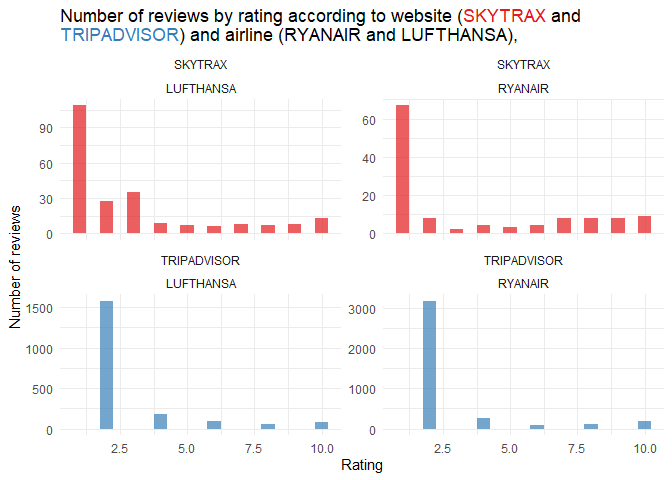
\includegraphics{index_files/figure-latex/notebooks-exploratory-analysis-fig-histogram-output-1.png}

}

\caption{\label{fig-histogram}Number of reviews by rating according to
website (`Skytrax' and `Tripadvisor') and airlines (Ryanair and
Lufthansa)}

\end{figure}%

\textsubscript{Source:
\href{https://chrglez.github.io/hierarchical_bayesian_airlines/notebooks/exploratory-analysis-preview.html\#cell-fig-histogram}{Exploratory
Analysis}}

Our analysis employs a standard 1--5 scale, with the Skytrax sample data
linearly transformed to match this conventional scale.

The histograms in Figure~\ref{fig-histogram} illustrate the frequency of
different review scores, showing a clear left skew (negative skewness)
in the distribution of scores for both airlines on both platforms. This
left skewness indicates that a majority of the reviews are clustered
towards the lower end of the rating scale. Specifically, a significant
number of reviews have scores of 1 or 2, while higher scores are less
frequent. This pattern suggests a tendency for customers to leave lower
ratings, which could be indicative of more frequent negative experiences
or higher expectations not being met.

\subsection{Bayesian Hierarchical
Model}\label{bayesian-hierarchical-model}

To analyze score heterogeneity, we applied a Bayesian hierarchical
model. Hierarchical models, also known as multilevel models, are useful
when data are structured in groups or clusters. In this study, reviews
are grouped by the site and airline. This hierarchical structure allows
us to account for the variability at both the site and airline levels.

Bayesian hierarchical models are powerful tools for analyzing data with
nested or grouped structures. These models have two main levels:

\begin{itemize}
\tightlist
\item
  \textbf{Fixed Effects}: These are the overall effects that apply to
  the entire population. In our study, the fixed effects include the
  site and airline.
\item
  \textbf{Random Effects}: These account for the variability within
  groups. In our study, the random effects capture the variability
  within each site and airline.
\end{itemize}

In our analysis, following Bianchi \& Heo (2021), we model the review
scores using a Poisson distribution.

\[
Pr(X\vert \lambda)=\frac{\exp{(-\lambda)}\lambda^x}{x!}
\]

This choice is appropriate because the scores are count data, which can
naturally be modeled using a Poisson distribution. The Poisson
distribution is widely used for modeling the number of events occurring
within a fixed interval of time or space when these events happen with a
known constant mean rate and independently of the time since the last
event. This fits well with the nature of review scores, which can be
considered as counts of discrete ratings.

The general form of a Bayesian hierarchical model can be expressed as:

\[
\text{score}_{ijk} \sim \text{Poisson}(\lambda_{ijk})
\]

\[
\log(\lambda_{ijk}) = \alpha + \beta_{i} + \gamma_{j} + \delta_{i \times j} + \epsilon_{ijk}
\]

Where:

\begin{itemize}
\tightlist
\item
  \(\lambda_{ijk}\) is the expected score for review \(k\) on site \(i\)
  for airline \(j\).
\item
  \(\alpha\) is the overall intercept.
\item
  \(\beta_{i}\) is the effect of site \(i\).
\item
  \(\gamma_{j}\) is the effect of airline \(j\).
\item
  \(\delta_{i \times j}\) is the interaction effect between site \(i\)
  and airline \(j\).
\item
  \(\epsilon_{ijk}\) is the random error term.
\end{itemize}

The results of the Bayesian hierarchical model applied to analyze the
heterogeneity of review scores are presented in \textbf{?@tbl-results}

::: \{\#tbl-results .cell tbl-alt=`Summary of Bayesian Hierarchical
Model Results including Fixed and Random Effects.' tbl-cap=' Summary of
Bayesian Hierarchical Model Results including Fixed (population-level)
and Random Effects (group-level).'\}

\begin{Shaded}
\begin{Highlighting}[]
\CommentTok{\#| label: tbl{-}results}
\CommentTok{\#| tbl{-}alt: "Summary of Bayesian Hierarchical Model Results including Fixed and Random Effects."}
\CommentTok{\#| tbl{-}cap: " Summary of Bayesian Hierarchical Model Results including Fixed (population{-}level) and Random Effects (group{-}level)."}

\NormalTok{fit }\SpecialCharTok{|\textgreater{}} \FunctionTok{tbl\_regression}\NormalTok{(}\AttributeTok{tidy\_fun =}\NormalTok{ broom.mixed}\SpecialCharTok{::}\NormalTok{tidy,}
                      \AttributeTok{intercept=}\ConstantTok{TRUE}\NormalTok{,}
                      \AttributeTok{estimate\_fun =} \SpecialCharTok{\textasciitilde{}} \FunctionTok{style\_sigfig}\NormalTok{(.x, }\AttributeTok{digits =} \DecValTok{3}\NormalTok{))}
\end{Highlighting}
\end{Shaded}

Characteristic

Beta

95\% CI

{1}

(Intercept)

1.05

-3.67, 6.17

site

~~~~SKYTRAX

---

---

~~~~TRIPADVISOR

-0.034

-4.65, 4.39

airline

~~~~LUFTHANSA

---

---

~~~~RYANAIR

0.144

-5.67, 5.87

site * airline

~~~~TRIPADVISOR * RYANAIR

-0.178

-0.299, -0.050

airline.sd\_\_(Intercept)

1.71

0.095, 4.84

site.sd\_\_(Intercept)

1.68

0.074, 5.02

{1}

CI = Credible Interval

\textsubscript{Source:
\href{https://chrglez.github.io/hierarchical_bayesian_airlines/notebooks/hierarchical-bayesian-model-preview.html\#ed1ee33f-b8ce-4ae3-b07a-78ed66be5581}{Hierarchical
Bayesian Model}}

Plot the results

:::

The overall intercept of 1.05 indicates the baseline level of review
scores when other factors are held constant. However, the wide 95\%
confidence interval ranging from -3.67 to 6.17 suggests high uncertainty
around this estimate, indicating that the baseline level can vary
significantly.

The effect of the site being TripAdvisor compared to Skytrax is
estimated at -0.03. This small effect size, coupled with a 95\%
confidence interval between -4.65 and 4.39, indicates that there is no
significant difference in review scores between TripAdvisor and Skytrax.
The wide confidence interval reflects substantial uncertainty and
variability in this comparison.

The effect of Ryanair compared to Lufthansa is estimated at 0.14.
Similar to the site effect, the 95\% confidence interval of -5.67 to
5.87 shows a wide range, indicating that there is no significant
difference in review scores between these two airlines. This suggests
that the review scores for Ryanair and Lufthansa are statistically
similar.

The interaction between the site TripAdvisor and the airline Ryanair is
estimated at -0.18, with a 95\% confidence interval from -0.30 to -0.05.
This negative interaction effect indicates that the combination of
TripAdvisor and Ryanair tends to have lower review scores compared to
other combinations. The narrow confidence interval suggests that this
interaction effect is statistically significant, implying a specific
negative effect when these two factors are combined.

The standard deviation of the intercept for the airlines is 1.71, with a
95\% confidence interval between 0.10 and 4.84. This indicates a
considerable amount of variability in the baseline review scores across
different airlines. The wide confidence interval suggests that while
there is some variability, the exact amount is uncertain.

The standard deviation of the intercept for the sites is 1.68, with a
95\% confidence interval between 0.07 and 5.02. Similar to the airline
intercept variability, this shows significant variability in the
baseline review scores across different sites. The wide confidence
interval reflects uncertainty in the extent of this variability.

\section{Conclusion}\label{conclusion}

This study explored the score heterogeneity of online consumer reviews
(OCRs) across two major airline review platforms---TripAdvisor and
Skytrax---using a Bayesian hierarchical model. Our findings provide
valuable insights into how review scores vary across different platforms
and airlines, contributing to the broader understanding of customer
feedback in the airline industry.

The analysis revealed no significant differences in review scores
between TripAdvisor and Skytrax or between Ryanair and Lufthansa. This
suggests that, on average, customer satisfaction as reflected in the
review scores is consistent across these platforms and airlines.
However, the interaction effect between TripAdvisor and Ryanair
indicates that specific platform-airline combinations can influence
customer perceptions, highlighting the nuanced nature of OCRs.

The significant variability in baseline scores across platforms and
airlines underscores the importance of considering both fixed and random
effects in understanding score heterogeneity. This finding aligns with
previous research (Bianchi \& Heo, 2021; Martel--Escobar et al., 2023),
emphasizing the need for robust statistical methods to manage the
diverse sources of OCR data.

Despite the strengths of our study, including the application of
advanced Bayesian hierarchical models, there are limitations that need
to be addressed. The analysis was constrained by the specific dataset,
which covered only one year of reviews for two airlines. Future research
should consider a broader dataset, including more airlines and a longer
timeframe, to validate and extend our findings.

Furthermore, the Bayesian hierarchical approach provides a framework for
incorporating prior knowledge and handling complex data structures,
making it a powerful tool for analyzing OCRs. However, further work is
needed to refine these models and explore their application in other
contexts within the tourism and hospitality sectors (Gómez-Déniz et al.,
2024).

In summary, our study contributes to the understanding of score
heterogeneity in OCRs and offers practical implications for airline
industry stakeholders. By highlighting the importance of
platform-airline interactions and the variability in customer feedback,
we provide insights that can help improve service quality and manage
brand reputation effectively. Future research should continue to explore
these dynamics, leveraging the strengths of Bayesian methodologies to
enhance our understanding of customer satisfaction in the digital age.

The findings of this study underscore the necessity for tailored
strategies in managing OCRs and provide a foundation for future research
in this area. By continuing to investigate the complex interactions
between review platforms, airlines, and customer perceptions, we can
develop more effective approaches to improving customer satisfaction and
fostering positive electronic word-of-mouth (eWOM) in the highly
competitive airline industry.

\section*{References}\label{references}
\addcontentsline{toc}{section}{References}

\phantomsection\label{refs}
\begin{CSLReferences}{1}{0}
\vspace{1em}

\bibitem[\citeproctext]{ref-assaker2020a}
Assaker, G. (2020). Age and gender differences in online travel reviews
and user-generated-content (UGC) adoption: Extending the technology
acceptance model (TAM) with credibility theory. \emph{Journal of
Hospitality Marketing and Management}, \emph{29}(4).
\url{https://doi.org/10.1080/19368623.2019.1653807}

\bibitem[\citeproctext]{ref-baka2016a}
Baka, V. (2016). The becoming of user-generated reviews: Looking at the
past to understand the future of managing reputation in the travel
sector. \emph{Tourism Management}, \emph{53}.
\url{https://doi.org/10.1016/j.tourman.2015.09.004}

\bibitem[\citeproctext]{ref-ban2019a}
Ban, H. J., \& Kim, H. S. (2019). Understanding customer experience and
satisfaction through airline passengers' online review.
\emph{Sustainability (Switzerland}, \emph{11}(15).
\url{https://doi.org/10.3390/su11154066}

\bibitem[\citeproctext]{ref-bianchi2021a}
Bianchi, G., \& Heo, C. Y. (2021). A bayesian statistics approach to
hospitality research. \emph{Current Issues in Tourism}, \emph{24}(22).
\url{https://doi.org/10.1080/13683500.2021.1896486}

\bibitem[\citeproctext]{ref-bilos2022a}
Bilos, A., Budimir, B., \& Hrustek, A. (2022). The role of
user-generated content in tourists' travel planning behavior: Evidence
from croatia. \emph{Journal of Tourism and Development}, \emph{39}.
\url{https://doi.org/10.34624/rtd.v39i0.27277}

\bibitem[\citeproctext]{ref-brochado2019a}
Brochado, A., Rita, P., Oliveira, C., \& Oliveira, F. (2019). Airline
passengers' perceptions of service quality: Themes in online reviews.
\emph{International Journal of Contemporary Hospitality Management},
\emph{31}(2). \url{https://doi.org/10.1108/IJCHM-09-2017-0572}

\bibitem[\citeproctext]{ref-brochado2023a}
Brochado, A., Duarte, M., \& Mengyuan, Z. (2023). Passengers'
perceptions of chinese airlines' service quality: A mixed methods
analysis of user-generated content. \emph{Journal of China Tourism
Research}, \emph{19}(3).
\url{https://doi.org/10.1080/19388160.2022.2122647}

\bibitem[\citeproctext]{ref-bronner2011a}
Bronner, F., \& Hoog, R. (2011). Vacationers and eWOM: Who posts, and
why, where, and what? \emph{Journal of Travel Research}, \emph{50}(1).
\url{https://doi.org/10.1177/0047287509355324}

\bibitem[\citeproctext]{ref-byun2016a}
Byun, H. J., \& Lee, B. C. (2016). Classifying service quality
attributes of low-cost carriers and full-service carriers based on an
analytical kano model. \emph{Global Business and Finance Review},
\emph{21}(2). \url{https://doi.org/10.17549/gbfr.2016.21.2.34}

\bibitem[\citeproctext]{ref-changchit2020a}
Changchit, C., Klaus, T., \& Lonkani, R. (2020). Online reviews: What
drives consumers to use them. \emph{Journal of Computer Information
Systems}. \url{https://doi.org/10.1080/08874417.2020.1779149}

\bibitem[\citeproctext]{ref-chatterjee2023a}
Chatterjee, S., Ghatak, A., Nikte, R., Gupta, S., \& Kumar, A. (2023).
Measuring SERVQUAL dimensions and their importance for
customer-satisfaction using online reviews: A text mining approach.
\emph{Journal of Enterprise Information Management}, \emph{36}(1).
\url{https://doi.org/10.1108/JEIM-06-2021-0252}

\bibitem[\citeproctext]{ref-cheong2008a}
Cheong, H. J., \& Morrison, M. A. (2008). Consumers' reliance on product
information and recommendations found in UGC. \emph{Journal of
Interactive Advertising}, \emph{8}(2).
\url{https://doi.org/10.1080/15252019.2008.10722141}

\bibitem[\citeproctext]{ref-cox2009a}
Cox, C., Burgess, S., Sellitto, C., \& Buultjens, J. (2009). The role of
user-generated content in tourists' travel planning behavior.
\emph{Journal of Hospitality and Leisure Marketing}, \emph{18}(8).
\url{https://doi.org/10.1080/19368620903235753}

\bibitem[\citeproctext]{ref-daugherty2008a}
Daugherty, T., Eastin, M. S., \& Bright, L. (2008). Exploring consumer
motivations for creating user-generated content. \emph{Journal of
Interactive Advertising}, \emph{8}(2).
\url{https://doi.org/10.1080/15252019.2008.10722139}

\bibitem[\citeproctext]{ref-davis1989a}
Davis, F. D. (1989). Perceived usefulness, perceived ease of use, and
user acceptance of information technology. \emph{MIS Quarterly:
Management Information Systems}, \emph{13}(3).
\url{https://doi.org/10.2307/249008}

\bibitem[\citeproctext]{ref-dike2024a}
Dike, S. E., Davis, Z., Abrahams, A., Anjomshoae, A., \& Ractham, P.
(2024). Evaluation of passengers' expectations and satisfaction in the
airline industry: An empirical performance analysis of online reviews.
\emph{Benchmarking}, \emph{31}(2).
\url{https://doi.org/10.1108/BIJ-09-2021-0563}

\bibitem[\citeproctext]{ref-etemad-sajadi2019a}
Etemad-Sajadi, R., \& Bohrer, L. (2019). The impact of service recovery
output/process on customer satisfaction and loyalty: The case of the
airline industry. \emph{Tourism and Hospitality Research}, \emph{19}(2).
\url{https://doi.org/10.1177/1467358417743080}

\bibitem[\citeproctext]{ref-filieri2018a}
Filieri, R., Hofacker, C. F., \& Alguezaui, S. (2018). What makes
information in online consumer reviews diagnostic over time? The role of
review relevancy, factuality, currency, source credibility and ranking
score. \emph{Computers in Human Behavior}, \emph{80}.
\url{https://doi.org/10.1016/j.chb.2017.10.039}

\bibitem[\citeproctext]{ref-filieri2019a}
Filieri, R., Raguseo, E., \& Vitari, C. (2019). What moderates the
influence of extremely negative ratings? The role of review and reviewer
characteristics. \emph{International Journal of Hospitality Management},
\emph{77}. \url{https://doi.org/10.1016/j.ijhm.2018.07.013}

\bibitem[\citeproctext]{ref-filieri2021a}
Filieri, R., Acikgoz, F., Ndou, V., \& Dwivedi, Y. (2021). Is
TripAdvisor still relevant? The influence of review credibility, review
usefulness, and ease of use on consumers' continuance intention.
\emph{International Journal of Contemporary Hospitality Management},
\emph{33}(1). \url{https://doi.org/10.1108/IJCHM-05-2020-0402}

\bibitem[\citeproctext]{ref-gomez2024a}
Gómez-Déniz, E., Martel-Escobar, M., \& Vázquez-Polo, F. J. (2024). A
bayesian model for online customer reviews data in tourism research: A
robust analysis. \emph{Cogent Business \& Management}, \emph{11}(1).
\url{https://doi.org/10.1080/23311975.2024.2363592}

\bibitem[\citeproctext]{ref-hassan2022a}
Hassan, T. H., \& Salem, A. E. (2022). Impact of service quality of
low-cost carriers on airline image and consumers' satisfaction and
loyalty during the covid-19 outbreak. \emph{International Journal of
Environmental Research and Public Health}, \emph{19}(1).
\url{https://doi.org/10.3390/ijerph19010083}

\bibitem[\citeproctext]{ref-hu2020a}
Hu, X., \& Yang, Y. (2020). What makes online reviews helpful in tourism
and hospitality? A bare-bones meta-analysis. \emph{Journal of
Hospitality Marketing and Management}.
\url{https://doi.org/10.1080/19368623.2020.1780178}

\bibitem[\citeproctext]{ref-huang2015a}
Huang, A. H., Chen, K., Yen, D. C., \& Tran, T. P. (2015). A study of
factors that contribute to online review helpfulness. \emph{Computers in
Human Behavior}, \emph{48}.
\url{https://doi.org/10.1016/j.chb.2015.01.010}

\bibitem[\citeproctext]{ref-jain2022a}
Jain, P. K., Patel, A., Kumari, S., \& Pamula, R. (2022). Predicting
airline customers' recommendations using qualitative and quantitative
contents of online reviews. \emph{Multimedia Tools and Applications},
\emph{81}(5). \url{https://doi.org/10.1007/s11042-022-11972-7}

\bibitem[\citeproctext]{ref-kaur2021a}
Kaur, K., \& Singh, T. (2021). What motivates consumers to write online
reviews? Qualitative research in the indian cultural context.
\emph{Journal of Global Marketing}, \emph{34}(3).
\url{https://doi.org/10.1080/08911762.2021.1882022}

\bibitem[\citeproctext]{ref-korfiatis2019a}
Korfiatis, N., Stamolampros, P., Kourouthanassis, P., \& Sagiadinos, V.
(2019). Measuring service quality from unstructured data: A topic
modeling application on airline passengers' online reviews. \emph{Expert
Systems with Applications}, \emph{116}.
\url{https://doi.org/10.1016/j.eswa.2018.09.037}

\bibitem[\citeproctext]{ref-kwok2016a}
Kwok, L., \& Xie, K. L. (2016). Factors contributing to the helpfulness
of online hotel reviews: Does manager response play a role?
\emph{International Journal of Contemporary Hospitality Management},
\emph{28}. \url{https://doi.org/10.1108/IJCHM-03-2015-0107}

\bibitem[\citeproctext]{ref-kwon2021a}
Kwon, H. J., Ban, H. J., Jun, J. K., \& Kim, H. S. (2021). Topic
modeling and sentiment analysis of online review for airlines.
\emph{Information Switzerland}, \emph{12}(2).
\url{https://doi.org/10.3390/info12020078}

\bibitem[\citeproctext]{ref-lam2020a}
Lam, J. M. S., Ismail, H., \& Lee, S. (2020). From desktop to
destination: User-generated content platforms, co-created online
experiences, destination image and satisfaction. \emph{Journal of
Destination Marketing and Management}, \emph{18}.
\url{https://doi.org/10.1016/j.jdmm.2020.100490}

\bibitem[\citeproctext]{ref-lim2020a}
Lim, J., \& Lee, H. C. (2020). Comparisons of service quality
perceptions between full service carriers and low cost carriers in
airline travel. \emph{Current Issues in Tourism}, \emph{23}(10).
\url{https://doi.org/10.1080/13683500.2019.1604638}

\bibitem[\citeproctext]{ref-lo2019a}
Lo, A. S., \& Yao, S. S. (2019). What makes hotel online reviews
credible?: An investigation of the roles of reviewer expertise, review
rating consistency and review valence. \emph{International Journal of
Contemporary Hospitality Management}, \emph{31}(1).
\url{https://doi.org/10.1108/IJCHM-10-2017-0671}

\bibitem[\citeproctext]{ref-lu2023a}
Lu, L., Xu, P., Wang, Y. Y., \& Wang, Y. (2023). Measuring service
quality with text analytics: Considering both importance and performance
of consumer opinions on social and non-social online platforms.
\emph{Journal of Business Research}, \emph{169}.
\url{https://doi.org/10.1016/j.jbusres.2023.114298}

\bibitem[\citeproctext]{ref-lu2015a}
Lu, W., \& Stepchenkova, S. (2015). User-generated content as a research
mode in tourism and hospitality applications: Topics, methods, and
software. \emph{Journal of Hospitality Marketing and Management},
\emph{24}(2). \url{https://doi.org/10.1080/19368623.2014.907758}

\bibitem[\citeproctext]{ref-lucini2020a}
Lucini, F. R., Tonetto, L. M., Fogliatto, F. S., \& Anzanello, M. J.
(2020). Text mining approach to explore dimensions of airline customer
satisfaction using online customer reviews. \emph{Journal of Air
Transport Management}, \emph{83}.
\url{https://doi.org/10.1016/j.jairtraman.2019.101760}

\bibitem[\citeproctext]{ref-martel2023a}
Martel--Escobar, M., González-Martel, C., \& Vázquez-Polo, F. J. (2023).
Managing score heterogeneity between online consumer review websites.
\emph{Cogent Social Sciences}, \emph{9}(2).
\url{https://doi.org/10.1080/23311886.2023.2267261}

\bibitem[\citeproctext]{ref-mendes-filho2018a}
Mendes-Filho, L., Mills, A. M., Tan, F. B., \& Milne, S. (2018).
Empowering the traveler: An examination of the impact of user-generated
content on travel planning. \emph{Journal of Travel and Tourism
Marketing}, \emph{35}(4).
\url{https://doi.org/10.1080/10548408.2017.1358237}

\bibitem[\citeproctext]{ref-migdadi2022a}
Migdadi, Y. K. A. A. (2022). The impact of airline alliance strategy on
the perceived service quality: A global survey. \emph{Journal of Quality
Assurance in Hospitality and Tourism}, \emph{23}(2).
\url{https://doi.org/10.1080/1528008X.2021.1884929}

\bibitem[\citeproctext]{ref-muda2021a}
Muda, M., \& Hamzah, M. I. (2021). Should i suggest this YouTube clip?
The impact of UGC source credibility on eWOM and purchase intention.
\emph{Journal of Research in Interactive Marketing}, \emph{15}(3).
\url{https://doi.org/10.1108/JRIM-04-2020-0072}

\bibitem[\citeproctext]{ref-muritala2020a}
Muritala, B. A., Sánchez-Rebull, M. V., \& Hernández-Lara, A. B. (2020).
A bibliometric analysis of online reviews research in tourism and
hospitality. \emph{Sustainability (Switzerland}, \emph{12}(ue 23)).
\url{https://doi.org/10.3390/su12239977}

\bibitem[\citeproctext]{ref-nicoli2017a}
Nicoli, N., \& Papadopoulou, E. (2017). TripAdvisor and reputation: A
case study of the hotel industry in cyprus. \emph{EuroMed Journal of
Business}, \emph{12}(3). \url{https://doi.org/10.1108/EMJB-11-2016-0031}

\bibitem[\citeproctext]{ref-nilashi2022a}
Nilashi, M., Abumalloh, R. A., Minaei-Bidgoli, B., Abdu Zogaan, W.,
Alhargan, A., Mohd, S., et al. (2022). Revealing travellers'
satisfaction during COVID-19 outbreak: Moderating role of service
quality. \emph{Journal of Retailing and Consumer Services}, \emph{64}.
\url{https://doi.org/10.1016/j.jretconser.2021.102783}

\bibitem[\citeproctext]{ref-nusairat2021a}
Nusairat, N. M., Alroale, M. A., Qeed, M. A., Al-Gasawneh, J. A.,
Hammouri, Q., Ahmad, A., \& Abdellatif, H. (2021). USER-GENERATED
CONTENT. \emph{Academy of Strategic Management Journal}, \emph{20}(4).

\bibitem[\citeproctext]{ref-park2020a}
Park, S., Lee, J. S., \& Nicolau, J. L. (2020). Understanding the
dynamics of the quality of airline service attributes: Satisfiers and
dissatisfiers. \emph{Tourism Management}, \emph{81}.
\url{https://doi.org/10.1016/j.tourman.2020.104163}

\bibitem[\citeproctext]{ref-punel2019a}
Punel, A., Al Hajj Hassan, L., \& Ermagun, A. (2019). Variations in
airline passenger expectation of service quality across the globe.
\emph{Tourism Management}, \emph{75}.
\url{https://doi.org/10.1016/j.tourman.2019.06.004}

\bibitem[\citeproctext]{ref-rasool2021a}
Rasool, G., \& Pathania, A. (2021). Reading between the lines: Untwining
online user-generated content using sentiment analysis. \emph{Journal of
Research in Interactive Marketing}, \emph{15}(3).
\url{https://doi.org/10.1108/JRIM-03-2020-0045}

\bibitem[\citeproctext]{ref-schuckert2015a}
Schuckert, M., Liu, X., \& Law, R. (2015). Hospitality and tourism
online reviews: Recent trends and future directions. \emph{Journal of
Travel and Tourism Marketing}, \emph{32}(5).
\url{https://doi.org/10.1080/10548408.2014.933154}

\bibitem[\citeproctext]{ref-sezgen2019a}
Sezgen, E., Mason, K. J., \& Mayer, R. (2019). Voice of airline
passenger: A text mining approach to understand customer satisfaction.
\emph{Journal of Air Transport Management}, \emph{77}.
\url{https://doi.org/10.1016/j.jairtraman.2019.04.001}

\bibitem[\citeproctext]{ref-siering2018a}
Siering, M., Deokar, A. V., \& Janze, C. (2018). Disentangling consumer
recommendations: Explaining and predicting airline recommendations based
on online reviews. \emph{Decision Support Systems}, \emph{107}.
\url{https://doi.org/10.1016/j.dss.2018.01.002}

\bibitem[\citeproctext]{ref-song2020a}
Song, C., Guo, J., \& Zhuang, J. (2020). Analyzing passengers' emotions
following flight delays- a 2011--2019 case study on SKYTRAX comments.
\emph{Journal of Air Transport Management}, \emph{89}.
\url{https://doi.org/10.1016/j.jairtraman.2020.101903}

\bibitem[\citeproctext]{ref-stamolampros2019a}
Stamolampros, P., Korfiatis, N., Kourouthanassis, P., \& Symitsi, E.
(2019). Flying to quality: Cultural influences on online reviews.
\emph{Journal of Travel Research}, \emph{58}(ue 3)).
\url{https://doi.org/10.1177/0047287518764345}

\bibitem[\citeproctext]{ref-sudhakar2020a}
Sudhakar, S., \& Gunasekar, S. (2020). Examining online ratings and
customer satisfaction in airlines. \emph{Anatolia}, \emph{31}(2).
\url{https://doi.org/10.1080/13032917.2020.1747238}

\bibitem[\citeproctext]{ref-sulu2022a}
Sulu, D., Arasli, H., \& Saydam, M. B. (2022). Air‐travelers'
perceptions of service quality during the COVID‐19 pandemic: Evidence
from TripAdvisor.com. \emph{Sustainability (Switzerland}, \emph{14}(1).
\url{https://doi.org/10.3390/su14010435}

\bibitem[\citeproctext]{ref-tahanisaz2020a}
Tahanisaz, S., \& shokuhyar, S. (2020). Evaluation of passenger
satisfaction with service quality: A consecutive method applied to the
airline industry. \emph{Journal of Air Transport Management}, \emph{83}.
\url{https://doi.org/10.1016/j.jairtraman.2020.101764}

\bibitem[\citeproctext]{ref-tsiakali2018a}
Tsiakali, K. (2018). User-generated-content versus
marketing-generated-content: Personality and content influence on
traveler's behavior. \emph{Journal of Hospitality Marketing and
Management}, \emph{27}(8).
\url{https://doi.org/10.1080/19368623.2018.1477643}

\bibitem[\citeproctext]{ref-ukpabi2018a}
Ukpabi, D. C., \& Karjaluoto, H. (2018). What drives travelers' adoption
of user-generated content? A literature review. In \emph{Tourism
management perspectives} (Vol. 28).
\url{https://doi.org/10.1016/j.tmp.2018.03.006}

\bibitem[\citeproctext]{ref-wang2023a}
Wang, X., Zheng, J., Tang, L., \& Luo, Y. (2023). Recommend or not? The
influence of emotions on passengers' intention of airline recommendation
during COVID-19. \emph{Tourism Management}, \emph{95}.
\url{https://doi.org/10.1016/j.tourman.2022.104675}

\bibitem[\citeproctext]{ref-wilson2012a}
Wilson, A., Murphy, H., \& Fierro, J. C. (2012). Hospitality and travel:
The nature and implications of user-generated content. \emph{Cornell
Hospitality Quarterly (Vol}, \emph{53}(ue 3)).
\url{https://doi.org/10.1177/1938965512449317}

\bibitem[\citeproctext]{ref-xu2019a}
Xu, X., Liu, W., \& Gursoy, D. (2019). The impacts of service failure
and recovery efforts on airline customers' emotions and satisfaction.
\emph{Journal of Travel Research}, \emph{58}(6).
\url{https://doi.org/10.1177/0047287518789285}

\bibitem[\citeproctext]{ref-yoo2009a}
Yoo, K. H., \& Gretzel, U. (2009). What motivates consumers to write
online travel reviews? \emph{Information Technology \& Tourism},
\emph{10}(4). \url{https://doi.org/10.3727/109830508788403114}

\end{CSLReferences}



\end{document}
